\subsection{Complexity of the simulation depending on the number of eigenvectors}

Throughout this section I will assume a lattice of size of $24^3 \times 48$.\\

\noindent
The complexity of the simulation increases linearly with the number of configurations. When changing the number of eigenvectors the simulation will be affected in different steps in a different way:

\begin{itemize}
    \item Naturally the time to calculate all eigenvectors depends \textbf{linearly} on the number of eigenvectors.
    \item The number of source and inverted source terms depends \textbf{linearly} on the number of eigenvectors as well. Therefore the same holds true for the time to calculate these.
    \item Computation times of the distilled gamma matrix increases \textbf{quadratically} with the number of eigenvectors.
    \item The time to calculate the perambulator depends quadratically on the number of source terms used and therefore also \textbf{quadratically} on the number of eigenvectors.
    \item As the last step the calculation of the correlation function depends on the number of eigenvectors \textbf{to the fourth}.
\end{itemize}

\begin{figure}[H]
        \centering
        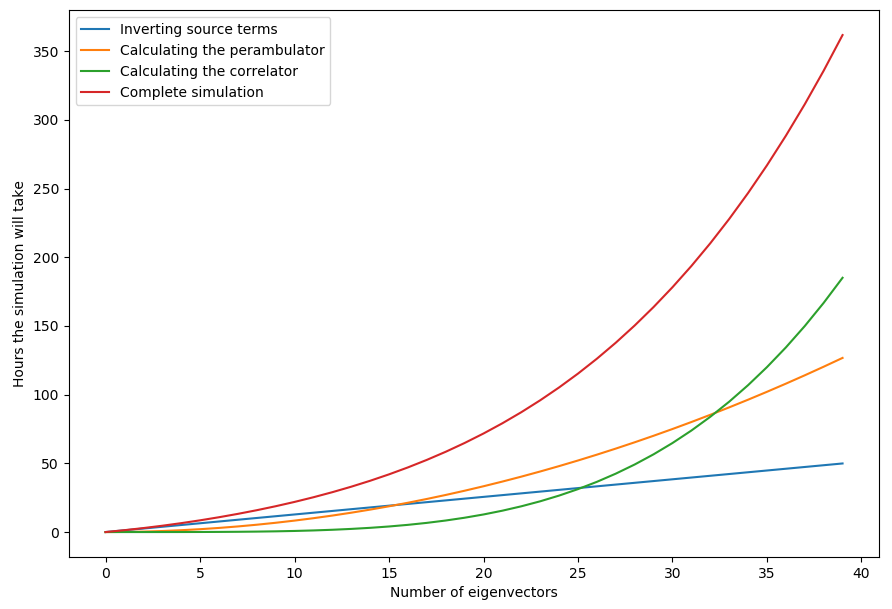
\includegraphics[width=1\textwidth]{images/time_of_sim.png}
        \caption{Distribution of the time the simulation will take}
        \label{time_of_sim}
    \end{figure}

\noindent
The inversion of the source terms usually takes the longest, followed by the computation of the perambulator. Calculating time for the eigenvectors, source terms and gamma matrix can be safely neglected. The correlator (with its $N^4$ dependence) on the other hand can also be neglected for small ($N<5$) number of eigenvectors but starts to play a major role when increasing the number of eigenvectors.

Inverting a single source term takes, when calculating the mass of a charmonium state, about 20 minutes per thread on the \textit{FUCHS} super computer. Calculating the perambulator for one eigenvector takes about 5 minutes. The last step, computing the correlator, needs for a single eigenvector circa 0.3 seconds. For the perambulator and correlator the time was calculated from the time each step takes when using 5 eigenvectors.

In figure \ref{time_of_sim} a plot of the time each of these steps will run for with respect to the number of eigenvectors can be seen.

This is of course a rough estimate, the actual time depends on a series of factors, e.g. differences between different computation nodes. It is also important to keep disc space constraints (ROM) in mind. The following table shows the space the files for each step need. One can see that the source terms will start to use a lot of disc space when using a higher number of eigenvectors. When computing the correlator with $N = 10$ on 11 configurations, all source terms combined used about 2.6TB of disc space.

\begin{table}[h]
            \centering
            \begin{tabular}{|c|c|}
            \hline
            \multicolumn{1}{|c|}{Step} & \multicolumn{1}{c|}{Approximate space needed} \\ \hline
             eigenvectors & 6MB $\times\ N$\\
             (inverted) source terms & 61MB $\times\ T \times 4 \times N$\\
             perambulator & 0.6MB $\times\ N^2$\\
             gamma matrix & 12KB $\times\ N^2$\\
             correlator & 37KB\\
              \hline
            \end{tabular}
            \caption{Disc space each step needs}
            \label{disc_space}
        \end{table}

\subsection{Outlook}

This work represents a first test of distillation by Marc Wagner's work group, therefore the number of eigenvectors and gauge configurations was kept small.

The results show that calculating meson masses using distillation is feasible. The particle in question is a light $\eta_c$ charmonium with a rest mass of $2983.4 \pm 0.5 \text{MeV}$ \cite{pdglive}. Even using only 11 gauge configurations a value close to that in the literature was observed. The results also show that a greater number of eigenvectors has a notable effect on the accuracy of the simulation. It appears preferably to use at least ten eigenvectors to reduce the error of the results. An increase of configuration will also play a large role in improving the simulation. Further tests will be needed to find a good balance between the number of eigenvectors and configurations.

Before attempting a computation of greater scale, a few improvements to the method can and should be made: Especially to reduce the space and time needed the source terms should be written into a single file. It probably has to be split again to be used by the inverter, but the computation of the perambulator will be sped up significantly if the program only needs to read one file into memory. Another step would be to utilize parallelism when computing the perambulator, eigenvectors and correlator.